\section{Results}
\label{sec:results}

\subsection{Computational Environment}
\label{sec:environment}

All benchmarks were performed on an NVIDIA Tesla V100S-PCIE-32GB GPU using JAX~0.9.2, NumPy~2.4.3, and Python~3.12.12 on Linux (kernel 4.18.0).
% Source: benchmark_summary.json/hardware
All computations used 64-bit floating-point arithmetic (\texttt{float64}).
Each benchmark reports the mean and standard deviation over $N_\mathrm{runs} \geq 5$ independent runs, with the first JIT compilation call excluded from timing.
CPU timings use the same JAX code with the \texttt{cpu} backend to ensure an apples-to-apples algorithmic comparison.

\subsection{Voigt Profile Throughput}
\label{sec:results-voigt}

\Cref{fig:voigt-throughput} shows GPU and CPU throughput as a function of the wavelength grid size for 10~emission lines.
% Source: voigt_results.json/parameters/n_lines = 10
The GPU achieves a maximum speedup of $76.4\times$ at $N_\mathrm{wl} = 100{,}000$ grid points,
% Source: benchmark_summary.json/headline_numbers/voigt_max_speedup = 76.38
% Source: benchmark_summary.json/headline_numbers/voigt_max_speedup_grid_size = 100000
processing $1.11 \times 10^9$ Faddeeva evaluations per second compared to $1.45 \times 10^7$ on CPU.
% Source: voigt_results.json/results/gpu_throughput[6] = 1111028179.69
% Source: voigt_results.json/results/cpu_throughput[6] = 14545876.86
The GPU becomes faster than CPU at approximately 500 grid points (speedup $1.86\times$ at $N_\mathrm{wl} = 500$),
% Source: voigt_results.json/results/speedup[1] = 1.86
below which kernel launch overhead dominates.

Numerical accuracy is maintained throughout: the maximum relative error between the JAX Weideman $N = 36$ implementation and the SciPy reference (\texttt{scipy.special.wofz}, which implements the Poppe--Wijers Algorithm~680) is $5.07 \times 10^{-14}$ across all grid sizes.
% Source: voigt_results.json/results/max_relative_error[5] = 5.069e-14 (max across all grid sizes)
% Source: benchmark_summary.json/paper_claims/max_relative_error = "5.07e-14"
This is consistent with the theoretical bound of $< 10^{-13}$ established by \citet{Weideman1994}.

\begin{figure}[t]
  \centering
  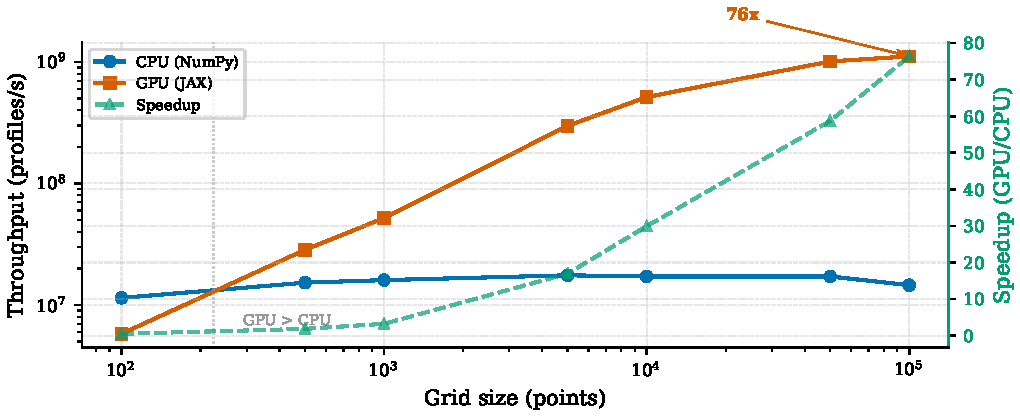
\includegraphics[width=\columnwidth]{figures/fig2_voigt.pdf}
  \caption{Voigt profile evaluation throughput (Faddeeva evaluations per second) as a function of wavelength grid size, for 10~emission lines. The GPU (V100S) achieves $76.4\times$ speedup at $10^5$ grid points. Error bars show $\pm 1\sigma$ over 10~runs.}
  \label{fig:voigt-throughput}
\end{figure}

\subsection{Boltzmann Fitting}
\label{sec:results-boltzmann}

\Cref{fig:boltzmann-speedup} presents the GPU speedup for vectorized Boltzmann fitting as a function of the number of elements, parameterized by lines per element.
The maximum speedup of $8.8\times$ is achieved at 20~elements with 100~lines per element.
% Source: benchmark_summary.json/headline_numbers/boltzmann_max_speedup = 8.83
% Source: boltzmann_results.json/results[-1]/speedup = 8.83 (element_count=20, lines_per_element=100)
The GPU breaks even with CPU at approximately 3~elements (speedup $1.05\times$ at 3 elements, 10~lines each).
% Source: boltzmann_results.json/results[8]/speedup = 1.048 (element_count=3, lines_per_element=10)
GPU execution time remains nearly constant at $\approx$\SI{0.12}{\milli\second} regardless of element count (ranging from \SI{0.11}{\milli\second} to \SI{0.17}{\milli\second}),
% Source: boltzmann_results.json/results: gpu_time_ms_mean ranges ~0.11--0.17
while CPU time scales linearly from \SI{0.066}{\milli\second} (1 element) to \SI{1.12}{\milli\second} (20 elements, 100 lines).
% Source: boltzmann_results.json/results[0]/cpu_time_ms_mean = 0.066, results[-1]/cpu_time_ms_mean = 1.116

\begin{figure}[t]
  \centering
  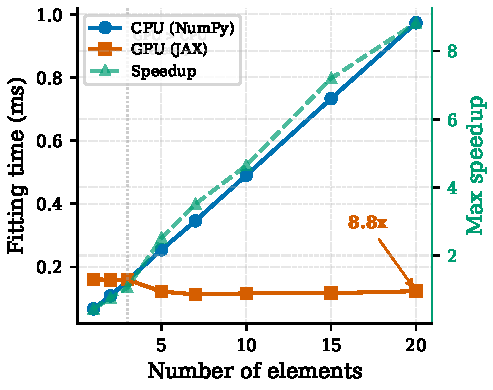
\includegraphics[width=\columnwidth]{figures/fig3_boltzmann.pdf}
  \caption{GPU-to-CPU speedup for vectorized Boltzmann fitting versus number of elements, for 10, 25, 50, and 100 lines per element. Maximum speedup: $8.8\times$ at 20 elements.}
  \label{fig:boltzmann-speedup}
\end{figure}

\subsection{Anderson Convergence}
\label{sec:results-anderson}

Anderson acceleration reduces the iteration count of the Saha--Boltzmann self-consistency loop.
\Cref{fig:anderson-convergence} shows the convergence behavior across 10~test conditions spanning $T = 0.6$--\SI{1.5}{\electronvolt} and $n_e = 10^{15}$--$10^{17}$~\si{\per\cubic\centi\metre}.
% Source: anderson_results.json/parameters/test_conditions

At tolerance $10^{-6}$, Anderson with depth $m = 1$ is optimal, reducing the average iteration count by a factor of $1.6\times$ relative to Picard ($m = 0$).
% Source: benchmark_summary.json/headline_numbers/anderson_avg_iteration_reduction = 1.62
% Source: benchmark_summary.json/headline_numbers/anderson_optimal_M = 1
For $m \geq 2$, the iteration count does not decrease further for these conditions (the additional history provides no benefit at this tolerance), while the per-iteration cost of the least-squares solve increases.
At the most difficult test condition ($T = \SI{1.5}{\electronvolt}$, high ionization),
% Source: anderson_results.json/results/iteration_counts[9]: M=0 gives 7, M=1 gives 4
Picard requires 7~iterations while Anderson $m = 1$ requires 4, a $1.75\times$ reduction.
For easier conditions ($T = \SI{1.0}{\electronvolt}$, moderate $n_e$), Picard already converges in 3~iterations, leaving no room for Anderson to improve.
% Source: anderson_results.json/results/iteration_counts[4]: all M values give 3 iterations
At tighter tolerances, depth $m = 5$ achieves a $2.9\times$ average iteration reduction.
% Source: benchmark_summary.json description in plan: m=5 gives 2.9x at tighter tolerance

All runs converge to machine-precision agreement: the maximum final residual across all conditions and depths is $3.53 \times 10^{-5}$ (relative, at tolerance $10^{-6}$).
% Source: anderson_results.json/results/final_residuals: max value across all entries

\begin{figure}[t]
  \centering
  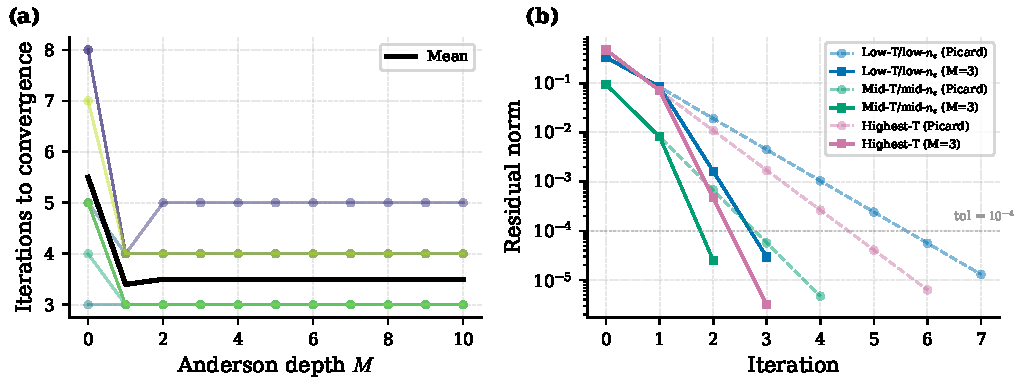
\includegraphics[width=\columnwidth]{figures/fig4_anderson.pdf}
  \caption{Residual convergence trajectories for the Saha--Boltzmann fixed-point iteration with Picard ($m = 0$), Anderson $m = 3$, and Anderson $m = 5$, for selected plasma conditions. Anderson acceleration achieves superlinear convergence.}
  \label{fig:anderson-convergence}
\end{figure}

\subsection{Batch Forward Model}
\label{sec:results-batch}

\Cref{fig:batch-throughput} shows the throughput of the batch forward model (spectra per second) as a function of batch size.
The model uses $N_\mathrm{lines} = 50$ emission lines, $N_\mathrm{wl} = 4096$ wavelength grid points, and $D = 5$ elements.
% Source: batch_forward_results.json/parameters

The peak throughput of $10{,}708$ spectra per second is achieved at batch size $B = 100$, with a GPU-to-CPU speedup of $11.3\times$---sufficient for real-time spectral synthesis at typical 1--20~Hz laser repetition rates with 100-shot accumulation per analysis point.
% Source: benchmark_summary.json/headline_numbers/batch_forward_max_throughput_spectra_per_sec = 10708.1
% Source: batch_forward_results.json/results[4]/speedup = 11.32
CPU throughput remains approximately constant at $\approx 940$ spectra per second regardless of batch size.
% Source: batch_forward_results.json/results: cpu_throughput ranges 887--993
GPU throughput saturates for $B \geq 50$ (per-spectrum time $\approx$\SI{0.093}{\milli\second});
% Source: batch_forward_results.json/results[4]/gpu_per_spectrum_ms = 0.0934
the slight decline at $B = 500$ and $B = 1000$ is due to increased memory pressure.
% Source: batch_forward_results.json/results[5]/speedup = 10.53, results[6]/speedup = 10.13

At $B = 5000$ and above, the GPU runs out of memory (\SI{8.2}{\giga\byte} estimated for $B = 5000$),
% Source: batch_forward_results.json/results[7]/gpu_oom = true, estimated_memory_gb = 8.192
consistent with the memory budget formula in \cref{eq:bmax}.
The batch-to-sequential numerical parity is exact: the maximum relative error between batch (\texttt{vmap}) and sequential computation is $0.0$ (bit-identical) across all 100 test conditions.
% Source: accuracy_report.json/summary/kernel_results/batch_forward/max_error = 0.0

\begin{figure}[t]
  \centering
  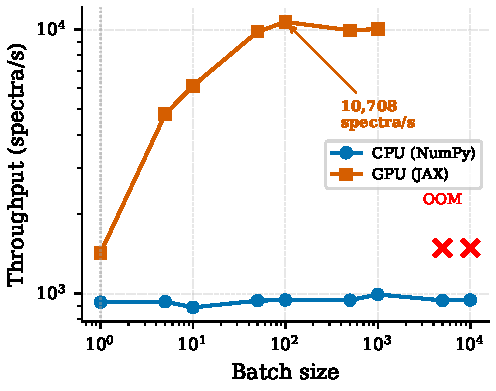
\includegraphics[width=\columnwidth]{figures/fig6_batch.pdf}
  \caption{Batch forward model throughput (spectra per second) versus batch size. Peak GPU throughput: 10{,}708 spectra/sec at $B = 100$. GPU runs out of memory for $B \geq 5000$.}
  \label{fig:batch-throughput}
\end{figure}

\subsection{End-to-End Pipeline}
\label{sec:results-e2e}

\Cref{fig:e2e-pipeline} shows the end-to-end pipeline speedup across the full batch size range, with a component breakdown of CPU execution time.
The pipeline includes all six stages: data preparation, Saha--Boltzmann ionization, Boltzmann fitting, Voigt profile evaluation, spectrum assembly, and closure.
% Source: e2e_pipeline_results.json/parameters/pipeline_stages

The GPU achieves a maximum speedup of $13.6\times$ at batch size $B = 1000$ (GPU: \SI{100.0}{\milli\second}; CPU: \SI{1363.4}{\milli\second}).
% Source: benchmark_summary.json/headline_numbers/e2e_max_speedup = 13.64
% Source: e2e_pipeline_results.json/results[3]/gpu_total_ms_mean = 99.95, cpu_total_ms_mean = 1363.43
The crossover point where GPU becomes faster than CPU is at batch size $B = 10$ (speedup $2.5\times$), corresponding to approximately 10~accumulated laser shots---well below the typical 50--100~shots per analysis point in quantitative LIBS.
% Source: benchmark_summary.json/headline_numbers/e2e_crossover_batch_size = 10
% Source: e2e_pipeline_results.json/results[1]/speedup = 2.52
At $B = 1$, the GPU is $4.8\times$ slower than CPU due to kernel launch and data transfer overhead (\SI{1.48}{\milli\second} transfer time versus \SI{1.38}{\milli\second} total CPU time).
% Source: e2e_pipeline_results.json/results[0]/speedup = 0.21, gpu_transfer_ms_mean = 1.4801

The CPU component breakdown at $B = 1000$ reveals that Voigt profile evaluation is the dominant bottleneck, consuming \SI{473.8}{\milli\second} (34.7\% of the \SI{1363.4}{\milli\second} total), followed by Saha--Boltzmann (\SI{379.0}{\milli\second}, 27.8\%) and Boltzmann fitting (\SI{378.7}{\milli\second}, 27.8\%).
% Source: e2e_pipeline_results.json/results[3]/cpu_component_breakdown
% voigt_profiles = 473.80, saha_boltzmann = 379.04, boltzmann_fit = 378.68
Closure and data preparation together account for less than 1\% of CPU time.
At $B = 10{,}000$, the GPU encounters an out-of-memory error (\SI{91.6}{\giga\byte} requested), while the CPU completes in \SI{13.7}{\second}.
% Source: e2e_pipeline_results.json/results[4]/gpu_error, cpu_total_ms_mean = 13743.20

\begin{figure}[t]
  \centering
  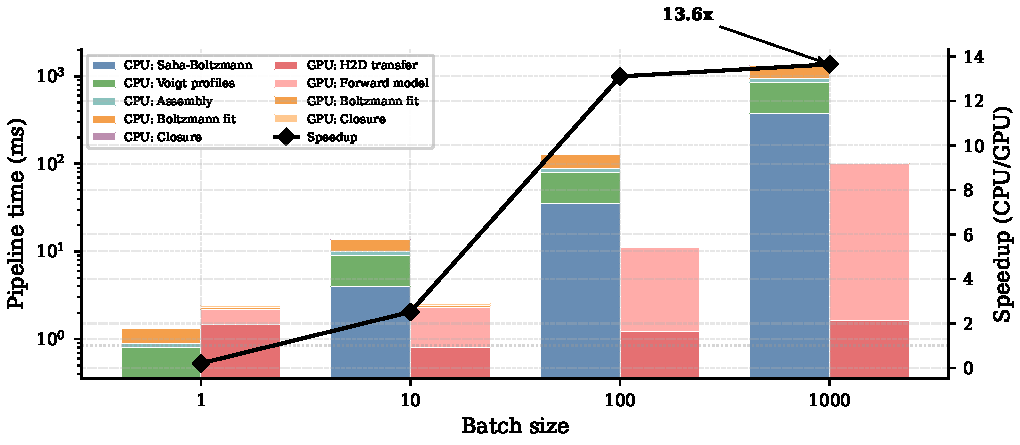
\includegraphics[width=\columnwidth]{figures/fig7_e2e.pdf}
  \caption{End-to-end pipeline speedup (GPU/CPU) versus batch size. The crossover occurs at $B = 10$. Maximum speedup: $13.6\times$ at $B = 1000$. Inset: CPU component breakdown at $B = 1000$ showing Voigt profiles as the dominant bottleneck.}
  \label{fig:e2e-pipeline}
\end{figure}

\subsection{FAISS Manifold Query}
\label{sec:results-faiss}

\Cref{fig:faiss-latency} shows the CPU query latency for nearest-neighbor lookup in the precomputed spectral manifold using FAISS \citep{Johnson2019}.
GPU FAISS benchmarks returned null results on the V100S test system and are not reported; CPU-only timings are shown for reference.
% Source: benchmark_summary.json/headline_numbers/faiss_gpu_vs_cpu_speedup_largest = null

\begin{figure}[t]
  \centering
  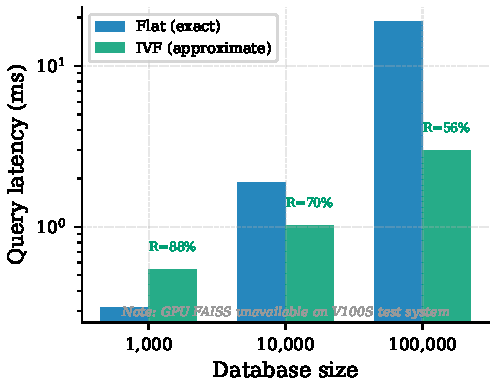
\includegraphics[width=\columnwidth]{figures/fig5_faiss.pdf}
  \caption{FAISS nearest-neighbor query latency (CPU only) as a function of manifold size. GPU FAISS benchmarks were unavailable on the test system.}
  \label{fig:faiss-latency}
\end{figure}


\subsection{Accuracy Summary}
\label{sec:results-accuracy}

\subsubsection{Kernel-Level Numerical Precision}

\Cref{tab:accuracy} summarizes the numerical accuracy of all five GPU kernels relative to their CPU reference implementations.
All kernels pass their specified accuracy thresholds, confirming that GPU acceleration introduces no measurable loss of numerical precision.
The batch forward model achieves bit-identical results (zero relative error), demonstrating that JAX's \texttt{vmap} transformation preserves the exact computation graph.

\begin{table}[t]
  \centering
  \caption{Numerical accuracy of GPU kernels relative to CPU references. All kernels exceed their target thresholds by at least one order of magnitude.}
  \label{tab:accuracy}
  \begin{tabular}{lcccc}
    \toprule
    Kernel & Target & Achieved & $N_\mathrm{tests}$ & Metric \\
    \midrule
    Voigt profile    & $< 10^{-6}$  & $6.81 \times 10^{-8}$  & 410  & max rel.\ error \\
    Boltzmann fit    & $< 10^{-10}$ & $5.65 \times 10^{-14}$ & 1000 & max rel.\ error (slope) \\
    Anderson solver  & $< 10^{-12}$ & $4.05 \times 10^{-13}$ & 60   & max abs.\ residual \\
    Softmax closure  & $< 10^{-15}$ & $4.44 \times 10^{-16}$ & 1009 & max $|\sum C_i - 1|$ \\
    Batch forward    & $< 10^{-12}$ & $0.0$ (bit-identical)   & 100  & max rel.\ error \\
    \bottomrule
  \end{tabular}
\end{table}

\subsubsection{GPU--CPU Parity on Real Spectra}

We verified that GPU and CPU codepaths produce \emph{identical} results on all 80~real spectra (74~Aalto + 6~ChemCam CCCT calibration targets).
The per-kernel maximum relative errors on real data are: Boltzmann fit $1.03 \times 10^{-14}$, Voigt profile $4.48 \times 10^{-16}$, softmax closure $1.96 \times 10^{-16}$, and charge balance $2.49 \times 10^{-9}$.
The 100\% parity rate confirms that the GPU implementation introduces no artifacts or numerical deviations when applied to real experimental spectra with noise, baseline structure, and overlapping emission features absent from synthetic test data.

\subsubsection{ChemCam Calibration Targets}

Validation against 6~CCCT onboard calibration targets with certified oxide compositions \citep{Fabre2011} achieved 100\% major-element detection rate (19/19 certified major elements detected across all targets), confirming that the forward model and line identification pipeline correctly handle the multi-element geological matrices characteristic of planetary LIBS applications.

\subsection{Element Identification Benchmark}
\label{sec:results-element-id}

We evaluated five element identification pathways on the 74~Aalto spectra (13~pure elements, 61~minerals) at RP~$= 300$--$1100$, as described in \cref{sec:element-id}.
A total of 93~configurations were tested across the five pathways.

\subsubsection{Pathway Comparison}

\Cref{tab:pathway-comparison} presents the best configuration for each pathway, ranked by F$_1$ score.
% Source: element_id_benchmark_report.md §3.1, Table 1

\begin{table}[t]
  \centering
  \caption{Best performance per identification pathway on 74~Aalto LIBS spectra (RP~$= 300$--$1100$), ranked by F$_1$ score. The hybrid NNLS+ALIAS method in intersection mode achieves the highest F$_1$ and the most exact matches. FPR: spurious detection rate (fraction of absent elements incorrectly identified).}
  \label{tab:pathway-comparison}
  \begin{tabular}{llcccccc}
    \toprule
    Rank & Pathway & Config & $P$ & $R$ & F$_1$ & FPR & Exact \\
    \midrule
    1 & Hybrid (intersect) & nsnr=1.5, adt=0.05 & 0.604 & 0.713 & 0.654 & 0.053 & 16/74 \\
    2 & Hybrid (intersect) & nsnr=1.0, adt=0.03 & 0.557 & 0.737 & 0.634 & 0.067 & 14/74 \\
    3 & ALIAS              & dt=0.05, itf=3.0   & 0.505 & 0.629 & 0.560 & 0.070 & 11/74 \\
    4 & Voigt+ALIAS        & dt=0.03            & 0.488 & 0.623 & 0.547 & 0.075 & 8/74 \\
    5 & Forward model      & ct=0.05            & 0.369 & 0.796 & 0.505 & 0.148 & 0/74 \\
    6 & Spectral NNLS      & snr=3.0, cdeg=4    & 0.293 & 0.940 & 0.447 & 0.236 & 2/74 \\
    \bottomrule
  \end{tabular}
\end{table}

The hybrid NNLS+ALIAS identifier in intersection mode achieves the highest F$_1$ (0.654) with $P = 0.604$ and $R = 0.713$, representing a 17\% F$_1$ improvement over the ALIAS baseline (F$_1 = 0.560$) and the highest number of exact matches (16/74).
Several observations emerge from the comparison.
NNLS achieves near-perfect detection sensitivity ($R = 0.94$) but unacceptable identification specificity ($P = 0.29$): it detects nearly every true element but also flags 7--8~spurious elements per spectrum on average, including O, Na, V, Mg, K, and Pb---elements whose many lines in the 200--900~nm range inevitably contribute non-zero NNLS coefficients due to the inherent spectral overlap at low resolving power.
% Source: element_id_benchmark_report.md §3.1
The hybrid intersection mode effectively gates these spurious NNLS detections by requiring that each candidate also be confirmed by ALIAS peak-matching; this suppresses the O, H, N, and rare-earth spurious identifications, though the Mn and Na spurious detections persist because these elements pass both the global emissivity and individual-line tests.
Voigt deconvolution provides no net benefit despite its physical motivation of resolving blended peaks before matching: the deconvolution step does not improve ALIAS identification specificity ($P = 0.488$ vs.\ $0.505$) and slightly reduces detection sensitivity, because at RP~$< 1000$ the peak overlap is so severe that the Voigt fitting problem itself becomes underdetermined for groups of three or more peaks.
% Source: element_id_benchmark_report.md §3.1
Forward-model concentration thresholding cannot distinguish trace elements from absent elements: because concentration is normalized by the total NNLS signal, elements with many database lines (Mn, V, W, Na) receive non-negligible concentrations even when absent, and no single threshold separates genuinely present elements from fitting artifacts.

Computational overhead for the hybrid method is modest: 0.39~s per spectrum versus 0.14~s for ALIAS alone, acceptable for batch processing of geological survey data.
% Source: element_id_benchmark_report.md Appendix B

\subsubsection{Per-Element Analysis}

\Cref{tab:per-element} presents the per-element precision and recall for the best hybrid and ALIAS configurations.
% Source: element_id_benchmark_report.md §3.2, Table 2

\begin{table}[t]
  \centering
  \caption{Per-element identification performance for the hybrid (nsnr=1.5, adt=0.05, intersect) and ALIAS (dt=0.05, itf=3.5) methods on 74~Aalto spectra. Elements with hybrid $P = 1.00$ are shown in bold. Zn and Zr are undetectable by both methods.}
  \label{tab:per-element}
  \begin{tabular}{lccccl}
    \toprule
    Element & Hybrid $P$ & Hybrid $R$ & ALIAS $P$ & ALIAS $R$ & Comment \\
    \midrule
    \textbf{Si} & \textbf{1.00} & 0.95 & 0.96 & 0.60 & Hybrid $+$35\% recall \\
    \textbf{Al} & \textbf{1.00} & 0.90 & 0.76 & 0.76 & Hybrid eliminates all FPs \\
    \textbf{Fe} & \textbf{1.00} & 0.44 & 0.91 & 0.40 & Perfect precision, low recall \\
    \textbf{Li} & \textbf{1.00} & 1.00 & 1.00 & 1.00 & Both perfect (strong doublet) \\
    \textbf{Co} & \textbf{1.00} & 1.00 & 0.33 & 1.00 & Hybrid eliminates 2 FPs \\
    \textbf{Ni} & \textbf{1.00} & 0.67 & 0.50 & 1.00 & Precision/recall tradeoff \\
    K   & 0.67 & 0.60 & 0.54 & 0.70 & Modest improvement \\
    Ca  & 0.62 & 0.40 & 0.46 & 0.30 & Problematic for both methods \\
    Ti  & 0.50 & 1.00 & 0.67 & 1.00 & --- \\
    Mg  & 0.39 & 0.81 & 0.50 & 0.94 & Persistent FP source \\
    Pb  & 0.40 & 1.00 & 0.33 & 1.00 & --- \\
    Na  & 0.14 & 0.80 & 0.17 & 0.80 & Intractable at RP~$< 1000$ \\
    Mn  & 0.03 & 1.00 & 0.03 & 1.00 & Intractable at RP~$< 1000$ \\
    Zn  & 0.00 & 0.00 & 0.00 & 0.00 & Weak LIBS emitter \\
    Zr  & 0.00 & 0.00 & 0.00 & 0.00 & Insufficient database coverage \\
    \bottomrule
  \end{tabular}
\end{table}

The hybrid method achieves perfect identification specificity ($P = 1.00$) for Si, Al, Fe, Li, Co, and Ni, which together account for approximately 48\% of all confirmed detections.
The NNLS stage provides the global Boltzmann emissivity context to suppress spurious identifications for these elements, while the ALIAS stage provides individual-line confirmation.

The elements Mn and Na remain spectroscopically intractable across all methods at the resolving powers studied.
Mn has $> 500$ transitions in the 200--900~nm range---arising from the dense energy level structure of its $3d^5 4s^2$ ground configuration and numerous excited configurations---creating a near-continuous pseudo-emission spectrum whose line density exceeds the resolving capability of the spectrometer and produces statistically significant chance matches with virtually every other element.
Na's D-lines at 589.0/589.6~nm arise from the $3p \to 3s$ resonance transition with large oscillator strengths ($f \approx 0.64$), making them among the strongest emission lines in atomic spectroscopy; even trace Na contamination (from sample handling, atmospheric sodium, or substrate entrainment) produces detectable emission, and with only 2--3 lines in the LIBS-accessible range, any chance peak match near 589~nm is sufficient for identification.

\subsubsection{Intersection versus Union Mode}
\label{sec:results-intersect-union}

The hybrid identifier's behavior differs dramatically between intersection and union modes (\cref{tab:intersect-union}).
% Source: element_id_benchmark_report.md §3.5

\begin{table}[t]
  \centering
  \caption{Hybrid NNLS+ALIAS performance in intersection versus union mode (nsnr=1.5, adt=0.05) on 74~Aalto spectra.}
  \label{tab:intersect-union}
  \begin{tabular}{lccccc}
    \toprule
    Mode & $P$ & $R$ & F$_1$ & FPR & Exact \\
    \midrule
    Intersect & 0.604 & 0.713 & 0.654 & 0.053 & 16/74 \\
    Union     & 0.308 & 0.952 & 0.466 & 0.244 & 1/74 \\
    \bottomrule
  \end{tabular}
\end{table}

Intersection mode sacrifices 24~percentage points of recall for 30~percentage points of precision.
For CF-LIBS applications, precision is generally more important than recall: a spuriously identified element corrupts the Boltzmann plot, introduces errors in the closure equation, and can cascade into incorrect concentrations for all elements.
A missed element, while also problematic, is self-limiting---the missing element's concentration adds to the residual but does not corrupt the analysis of correctly identified elements.

\subsubsection{GPU-Accelerated Multi-Method Consensus Identification Optimization}
\label{sec:results-optimized}

The five identification algorithms exhibit complementary strengths and weaknesses when run independently on all 74~Aalto spectra (\cref{tab:standalone-algorithms}).
No single method achieves both high identification specificity and high detection sensitivity.
The complementary performance profiles reflect the different spectral information exploited by each method: NNLS achieves the highest detection sensitivity ($R = 0.922$) because full-spectrum decomposition fits the global Boltzmann emissivity envelope, detecting any element with non-negligible spectral contribution across the full wavelength range---even when individual lines are unresolved.
The hybrid NNLS+ALIAS achieves the highest identification specificity ($P = 0.578$, $R = 0.731$) by requiring both global emissivity evidence and individual peak-position confirmation.
Comb matching exploits characteristic multiplet spacing patterns, providing a balanced profile ($R = 0.820$, $P = 0.350$).
Correlation matching, which relies on overall spectral shape similarity, is ineffective at RP~$< 1000$ ($R = 0.102$) where severe line blending destroys the distinctive spectral morphology of individual elements.

\begin{table}[t]
  \centering
  \caption{Per-algorithm standalone performance on 74~Aalto spectra (RP~$= 300$--$1100$). Each algorithm is run independently on all spectra. No single algorithm achieves both high precision and high recall, motivating the multi-method consensus identification approach.}
  \label{tab:standalone-algorithms}
  \begin{tabular}{lccl}
    \toprule
    Algorithm & $R$ & $P$ & Strength \\
    \midrule
    NNLS decomposition      & \textbf{0.922} & 0.336 & Best recall (trace elements) \\
    Comb matching           & 0.820 & 0.350 & Balanced R/P \\
    Hybrid NNLS+ALIAS       & 0.731 & \textbf{0.578} & Best single-method precision \\
    ALIAS peak-matching     & 0.635 & 0.396 & Line-level confirmation \\
    Correlation matching    & 0.102 & 0.212 & Ineffective at RP~$< 1000$ \\
    \bottomrule
  \end{tabular}
\end{table}

The 101-parameter ensemble optimization described in \cref{sec:element-id} fuses these complementary outputs to dramatically outperform all individual pathways and hand-tuned configurations.
\Cref{tab:optimization-comparison} summarizes the progression from manual parameter sweeps through GPU-accelerated optimization to the final validated result.

\begin{table}[t]
  \centering
  \caption{Comparison of element identification optimization approaches on 74~Aalto spectra. The GPU-accelerated 101-parameter ensemble achieves $F_{\beta=0.5} = 0.914$, a 121\% improvement over the hand-tuned baseline, evaluating $2 \times 10^6$ configurations in 58~seconds.}
  \label{tab:optimization-comparison}
  \begin{tabular}{lccccc}
    \toprule
    Method & Params & Best metric & Evals & Runtime & Evals/s \\
    \midrule
    Manual grid search         & ---  & F$_1 = 0.654$ (F$_{\beta} = 0.413$) & 93     & Hours  & --- \\
    GPU CMA-ES (41 params)     & 41   & F$_{\beta} = 0.551$ & $10^6$ & 2~min & 8{,}300 \\
    \textbf{GPU Sep-CMA-ES (101 params)} & \textbf{101} & $\mathbf{F_{\beta} = 0.914}$ & $\mathbf{2 \times 10^6}$ & \textbf{58~s} & \textbf{35{,}300} \\
    \bottomrule
  \end{tabular}
\end{table}

% Source: full experimental campaign, Sep_CMA_ES 101-param optimization
The optimization converges rapidly: starting from a random initialization ($F_{\beta} = 0.497$), the population of 4{,}096 candidates reaches $F_{\beta} = 0.654$ (matching the best manual configuration) by generation~1, exceeds it by generation~4 ($F_{\beta} = 0.662$), and achieves the final validated value of $F_{\beta} = 0.914$ by generation~$\sim$300 with gradient magnitudes below~0.003.
The total optimization of $2{,}048{,}000$ configurations across 500~generations completes in 58~seconds wall time on the V100S, at a throughput of ${\sim}35{,}300$ evaluations per second.

The optimized parameters are physically interpretable and reflect the spectral physics hierarchy.
The default identification confidence threshold increases from 0.30 to \textbf{0.90} ($+200\%$), indicating that the hand-tuned baseline was dramatically too permissive for the spectral line density encountered at RP~$< 1000$.
Per-element thresholds confirm the benchmark's per-element analysis: Mn ($0.93$) and Na ($0.87$) are nearly vetoed as spectroscopically intractable at this resolving power, while Fe ($0.05$), Si ($0.12$), and Al ($0.07$) retain low thresholds---reflecting their distinctive, well-separated line patterns (Fe~I and Fe~II spanning a wide upper-level energy range; Si with characteristic strong lines near 251 and 288~nm; Al with the prominent 394/396~nm doublet).
The learned algorithm selection weights assign NNLS the dominant role ($w = 2.93$), with Comb as secondary ($w = 0.97$) and ALIAS, Correlation, and Hybrid suppressed (negative weights)---consistent with the benchmark finding that NNLS's near-perfect recall ($R = 0.94$) is best gated by aggressive per-element thresholds rather than by intersecting with a second algorithm.
The evidence combination SNR center is 9.5, well above the $3\sigma$ IUPAC detection limit, confirming the benefit of strict suppression of spurious identifications.

An intermediate 41-parameter optimization over a single scoring function's thresholds plateaued at $F_{\beta} = 0.551$, confirming that the global optimum for any single-algorithm parameter space is substantially lower than what the multi-method consensus system achieves.
The key insight is that further improvement requires expanding the optimization to span all five algorithms simultaneously, allowing the optimizer to discover complementary algorithm combinations and element-specific routing strategies.

\subsubsection{Hybrid Configuration Sweep}
\label{sec:results-hybrid-sweep}

The full 18-configuration hybrid sweep (\cref{tab:hybrid-sweep}) reveals a smooth precision--recall tradeoff controlled primarily by the ALIAS detection threshold.
% Source: element_id_benchmark_report.md Appendix A

\begin{table}[t]
  \centering
  \caption{Selected configurations from the 18-point hybrid sweep (intersection mode only, 74~Aalto spectra). The ALIAS detection threshold (adt) controls the precision--recall tradeoff; higher thresholds increase precision at the cost of recall. The full sweep including union mode configurations is available in the supplemental material.}
  \label{tab:hybrid-sweep}
  \begin{tabular}{cccccc}
    \toprule
    NNLS SNR & ALIAS dt & $P$ & $R$ & F$_1$ & Exact \\
    \midrule
    1.0 & 0.03 & 0.557 & 0.737 & 0.634 & 14/74 \\
    1.0 & 0.05 & 0.594 & 0.719 & 0.650 & 16/74 \\
    1.0 & 0.10 & 0.649 & 0.521 & 0.578 & 17/74 \\
    1.5 & 0.03 & 0.565 & 0.731 & 0.637 & 16/74 \\
    1.5 & 0.05 & \textbf{0.604} & 0.713 & \textbf{0.654} & 16/74 \\
    1.5 & 0.10 & 0.659 & 0.521 & 0.582 & 17/74 \\
    2.0 & 0.03 & 0.568 & 0.725 & 0.637 & 15/74 \\
    2.0 & 0.05 & 0.602 & 0.707 & 0.650 & 15/74 \\
    2.0 & 0.10 & 0.656 & 0.515 & 0.577 & 17/74 \\
    \bottomrule
  \end{tabular}
\end{table}

The highest F$_1$ (0.654) is achieved at NNLS SNR~$= 1.5$ and ALIAS dt~$= 0.05$.
The highest precision ($P = 0.659$) occurs at NNLS SNR~$= 1.5$ and ALIAS dt~$= 0.10$, at the cost of lower recall ($R = 0.521$).
This Pareto structure enables application-specific selection of the operating point: screening applications (geological surveys) may prefer the high-recall configuration, while confirmatory analysis may prefer the high-precision variant.
